\documentclass[numbers=noenddot,10pt,a4paper]{scrartcl}
\usepackage[greek,ngerman]{babel}
\usepackage[T1]{fontenc}
\usepackage[utf8]{inputenc}
\usepackage{fullpage}
\usepackage{libertine}
\usepackage{ziffer}
\usepackage{graphicx}
\usepackage{units}
%\usepackage{wasysym}
\usepackage{amsmath}
\usepackage{amssymb}
\usepackage{wrapfig}
\usepackage{esint}
\usepackage{float}
\usepackage{wrapfig}
\usepackage[font=small]{caption}
\usepackage{subcaption}

\renewcommand{\thefigure}{Abb. \arabic{figure}}

\captionsetup[wrapfigure]{name=}
\captionsetup[figure]{name=}
\newcommand{\degree}{^\circ}
\newcommand{\diff}{\textnormal{d}}
\newcommand{\tenpo}[1]{\cdot 10^{#1}}
\newcommand{\greek}[1]{\greektext#1\latintext}
\newcommand{\indx}[1]{_\text{#1}}

\title{Protokoll: Astabiler Multivibrator}
\author{Tom Kranz, Philipp Hacker}
\date{\today}

\begin{document}
%\setcounter{page}{2}
%\setcounter{section}{1}
\maketitle
\vspace*{\fill}
\tableofcontents
\vfill
\newpage
\section{Vorbereitung}
\subsection{Schaltskizzen}
\begin{figure}[H]
\centering
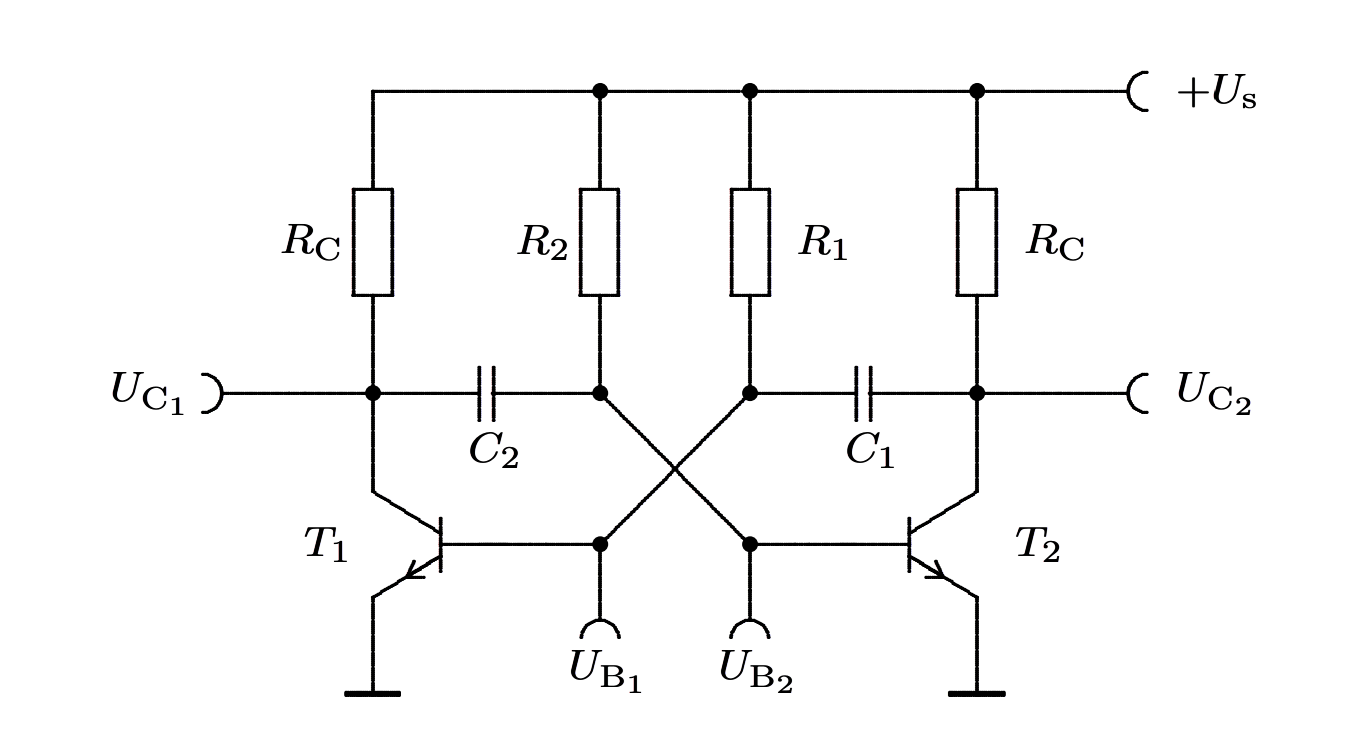
\includegraphics[width=0.75\textwidth]{schaltskizze1}
\caption{Astabiler Multivibrator}
\end{figure}
\begin{figure}[H]
\centering
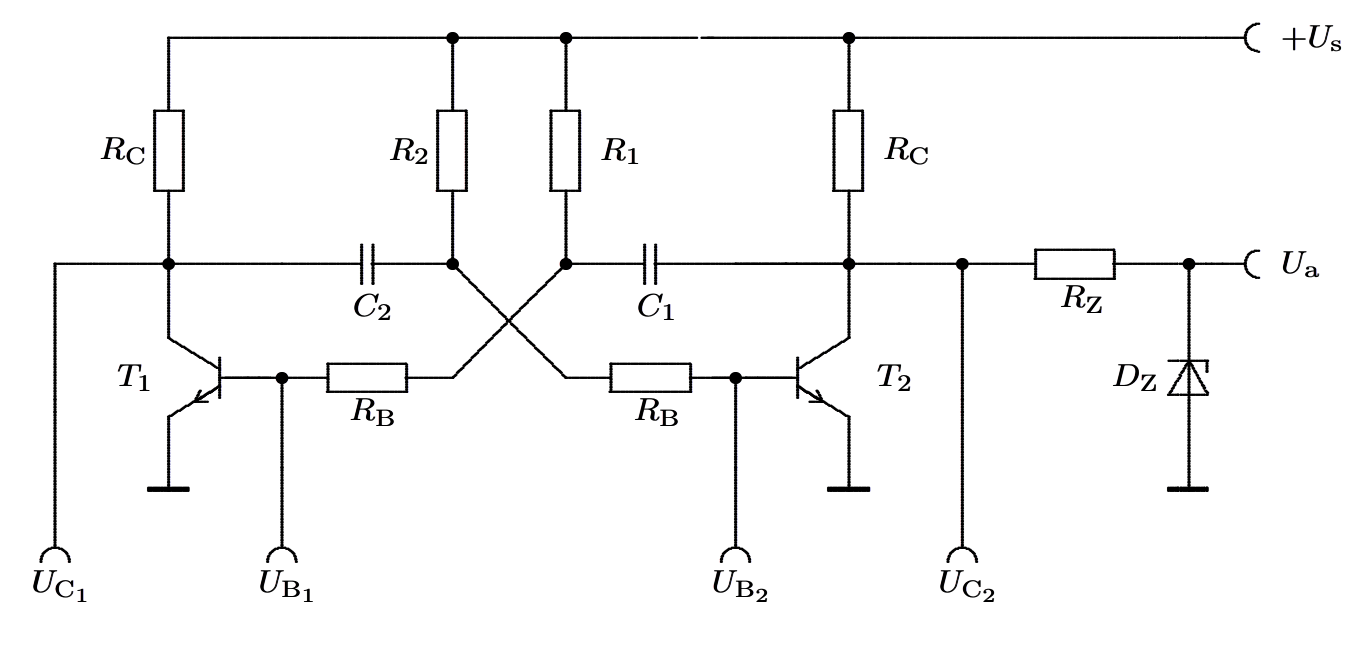
\includegraphics[width=0.75\textwidth]{schaltskizze2}
\caption{Astabiler Multivibrator mit Transistorvorwiderständen und Zener-Diode über dem Ausgang}
\end{figure}
\subsection{Berechnungsaufgabe 1 - korrigierte Frequenz}
Es gilt, dass
\begin{align}
U\indx{B}(t=0)=U\indx{BE;sat}-(U\indx{S}-U\indx{CE;sat}) \quad \text{und} \quad U\indx{B}(t\indx{2})=U\indx{BE;Schw} \, .
\end{align}
Somit folgt für die Funktion der Basisspannung $U\indx{B}(t)$, mit den Zeitkostanten $\tau_i=R_i\cdot C_i$:
\begin{align}
U\indx{B}(t)=U\indx{B}(t=0)+(U\indx{S}-U\indx{B}(t=0))\cdot\left(1-\exp\left(-\frac{t}{\tau\indx{2}}\right)\right) \, .
\end{align}
Zum Zeitpunkt $t\indx{2}$ ist also
\begin{align}
U\indx{BE;Schw}=U\indx{B}(t=0)+(U\indx{S}-U\indx{B}(t=0))\cdot\left(1-\exp\left(-\frac{t\indx{2}}{\tau\indx{2}}\right)\right) \, .
\end{align}
Nach Umformung analog zur Praktikumsanleitung, Gleichungen (1.3) und folgende, steht:
\begin{align}
t\indx{2}=-\tau\indx{2}\ln\left(\frac{2\cdot U\indx{S}-U\indx{BE;sat}-U\indx{CE;sat}}{U\indx{S}-U\indx{BE,sat}}\right)
\end{align}
Für den Zeitpunkt $t'=t\indx{3}-t\indx{2}$ gilt ähnliches, wobei $t\indx{3}$ der Periodendauer $T$ entspricht. Somit folgt
\begin{align}
t_3-t_2=\tau_1 \ln\left(\frac{2\cdot U\indx{S}-U\indx{BE;sat}-U\indx{CE;sat}}{U\indx{S}-U\indx{BE,sat}}\right) \, .
\end{align}
Schließlich steht
\begin{align}
t_3=\frac{1}{f}=(\tau_1+\tau_2)\ln\left(\frac{2\cdot U\indx{S}-U\indx{BE;sat}-U\indx{CE;sat}}{U\indx{S}-U\indx{BE,sat}}\right) \, .
\end{align}
\subsection{Berechnung 2 - Dimensionierung}
Es war eine Frequenz von ungefähr $\unit[5]{kHz}$ angestrebt. Dafür sollten $R_1=R_2$ und $C_1=C_2$ angepasst werden, wobei darauf geachtet werden musste, dass der Strom durch die Widerstände zum vollkommenen Durchsteuern der Transistoren genügt, aber nicht so groß ist, dass über den Widerständen gefährlich hohe Leistung abfällt. Des Weiteren musste $R_C$ genügend klein sein, um die Stromverstärkung des Transistors voll auszureizen.
\section{Durchführung}
\section{Auswertung}
\section{Quellen}
\section{Anhang}
\subsection{Messwerte}
Die originalen Messwert-Aufzeichnungen liegen bei.
\end{document}